\documentclass[12pt,fleqn]{article}\usepackage{../../common}
\begin{document}
Sıvılar, Hava, Hava Dinamiği

Süreklilik Denklemi

Farklı noktalarda boyutları farklı olan bir tüp içinde istikrarlı akış
içindeki bir sıvının $v$ ve $A$ ifadelerini birbiriyle ilintilendiren bir
formül kurmak istiyoruz. Bir $t$ zamanından başlayarak $\Delta t$ kadar
süre içindeki tüpün solunda oluşan hacim ve bu hacmin dışarı itmesi
gereken, eğer sıvı sıkıştırılamaz ise, eşit bir hacim vardır. Soldan
$\Delta V$ girmişse $\Delta V$ çıkmalıdır. 

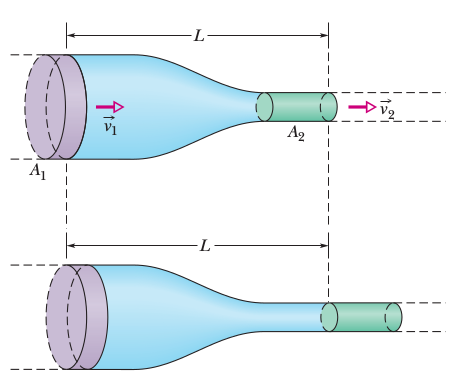
\includegraphics[width=20em]{phy_045_flight_01.png}

Genel bağlamda $\Delta x = v \Delta t$ ise,

$$
\Delta V = A \Delta x = A v \Delta t
$$

Şimdi tüpün solu ve sağı özelinde,

$$
\Delta V = A_1 v_1 \Delta t = A_2 v_2 \Delta t
$$

$$
A_1 v_1 = A_2 v_2
$$

Üstteki denkleme süreklilik denklemi adı veriliyor.

Bu denklemi 

$$
R_V = A v = \textrm{sabit}
$$

olarak ta yazabiliriz, çünkü süreklilik denklemi herhangi iki nokta için
doğru olmalıdır, o zaman üstteki ifade de geçerlidir. $R_V$'ye hacim akış
oranı denir. 

Ek olarak sıvının yoğunluğu her yerde eşit ise, mesela $\rho$ diyelim, o
zaman 

$$
R_m = \rho R_v = \rho A v = \textrm{sabit}
\mlabel{3}
$$

sonucuna da varılabilir [1, sf. 399].


Bernoulli Deklemi

İstikrarlı akış halindeki bir sıvıyı düşünelim, alttaki resimdeki gibi
yandan görülen bir tüpte / boruda akıyor. Diyelim ki 1. resim ile 2. resim
arasında geçen zaman $\Delta t$ ve o zaman içinde koyu mavi olan bölüm
kadar sıvı hacmi yer değiştiriyor [1, sf 402].

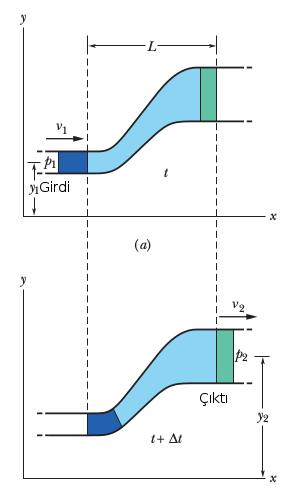
\includegraphics[width=20em]{phy_045_flight_02.png}

Bu değişimin tüp sonunda yeşil bölge kadar hacim değişikliğine yol
açar diyelim, ve önemli bir nokta iki hacim birbirine eşittir.  Eğer
1. resimdeki sıvının girişteki yükseklik, hız, ve basıncı
$y_1,v_1,p_1$ ile temsil ediliyorsa, 2. resimde diğer uçtaki
$y_2,v_2,p_2$ diyelim, bu değişkenler

$$
p_1 + \frac{1}{2} \rho v_1^2 + \rho g y_1 =
p_2 + \frac{1}{2} \rho v_2^2 + \rho g y_2 
\mlabel{1}
$$

formülü ile birbiriyle bağlıdır, ki $\rho$ sıvı yoğunluk
sabiti. Üstteki denklemi

$$
p + \frac{1}{2} \rho v^2 + \rho g y = \textrm{bir sabit}
\mlabel{2}
$$

olarak ta yazabiliriz. Bu son formül Bernoulli'nin formülüdür, onun
daha yaygın bilinen formudur.

Formüle erişmek için iş-kinetik enerji teorisinden başlayabiliriz, 

$$
W = \Delta K
$$

Yapılan iş kinetik enerjideki değişime eşittir. Sıvı için kinetik enerji
değişimi sıvının tüp başında ve sonundaki hızı ile alakalı olmalıdır [1,
sf. 403],

$$
\Delta K = \frac{1}{2} \Delta m v_2^2 - \frac{1}{2} \Delta m v_1^2 
$$

ki $\Delta m$ tüpün başında $\Delta t$ anında içeri giren sıvı kütlesi. Onu
$\Delta m = \rho \Delta V$ olarak ta yazabiliriz ki $\Delta V$ aynı zaman
aralığında giren sıvı hacmi.

$$
= \frac{1}{2} \rho \Delta V(v_2^2 - v_1^2)
$$

Şimdi basıncı dahil edelim, bu da bir kuvvet, tüpün başında pozitif iş
yapıyor, sonunda içerideki tüm sıvının kütlesi üzerinden ters yönde iş
yapıyor, genel olarak 

$$
F \Delta x  = (pA)(\Delta x) = p(A\Delta x) = p \Delta V
$$

denebilir, o zaman baştaki iş $p_1 \Delta V$, sondaki iş $p_2 \Delta V$,
toplam

$$
W_p = -p_2 \Delta V + p_1 \Delta V
$$

$$
= - (p_2-p_1) \Delta V
$$

Yerçekimin yaptığı iş negatiftir, $W_g$ diyelim, kuvvet çarpı yer
değişikliği. Kuvvet $\Delta m g$, yer değişikliği $y_2-y_1$. 

$$
W_g = -\Delta m g (y_2 - y_1)
$$

$$
= -\rho g \Delta V (y_2-y_1)
$$


Hepsini bir araya koyarsak, yapılan iş eşittir kinetik enerji değişimi
üzerinden,

$$
W = W_g + W_p = \Delta K
$$

$$
-\rho g \Delta V(y_2-y_1) - \Delta V(p_2-p_1) = 
\frac{1}{2} \rho \Delta V(v_2^2 - v_1^2)
$$

Tekrar düzenlersek (1)'e erisebiliriz. (2) denklemi (1)'e bakmanın bir
diğer yönü, çünkü aslında (2) diyor ki basınç $P$ artı kinetik enerji
$\frac{1}{2} \rho v^2$ artı yerçekimsel potansiyel enerji yoğunluğu
$\rho g y$'yi tüp akışındaki herhangi iki noktada hesaplarsak birbirlerine
eşit olmalılar. O zaman, $p + \frac{1}{2} \rho v^2 + \rho g y$ formülü her
noktada aynı olacağına göre bu ifadenin bir sabite eşit olduğu da
söylenebiliyor. Yani

$$
p + \frac{1}{2} \rho v^2 + \rho g y = \textrm{bir sabit}
$$

oluyor. Diğer bir yoden bakarsak, üstteki formüle bir enerji denklemi de
denebilir. Tüm formülü $\rho$ ile bölersek,

$$
\frac{p}{\rho} + \frac{1}{2} v^2 + gh = \textrm{sabit}
$$

Burada $p\rho$ basic enerjisi, $\frac{1}{2}v^2$ kinetik enerji, $gy$ ise
potansiyel enerji. Bir sıvı (ya da aerodinamik durumunda hava) ögesi,
parçacığı bir tüpte akarken toplam enerjisinin muhafaza eder. 

Bir hava taşıtının etrafından akan hava durumunda öğelerin dikey yer
değişimi genellikle çok küçüktür o zaman yok sayılabilirler, bu durumda
Bernoulli denklemi 

$$
p + \frac{1}{2} \rho v^2 = \textrm{sabit}
$$

formuna indirgenebilir [3, sf 97]. 

Helikopter

Bir helikopterin pervanesi dönerken üstteki hava parçacıklarını alıp aşağı
doğru iter. Olanları sanki bir tüp içinde sıvı akışıymış gibi görebiliriz,
ama ufak bir fark var, altta dikey çizgiyle gösterilen (yandan bakış)
pervane sıvıya, daha doğrusu havaya bir enerji ekler.

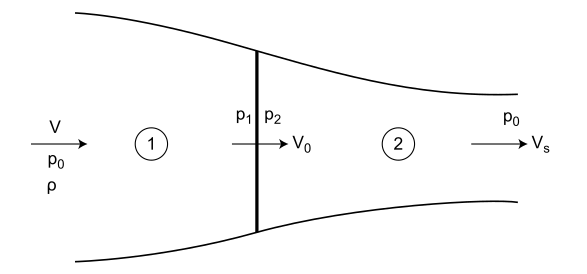
\includegraphics[width=25em]{phy_045_flight_03.png}

Bu sebeple bir enerji hesabı yapmak istiyorsak Bernoulli denklemini iki
bölgeye ayrı ayrı uygulamamız gerekir. Pervane öncesi, ve sonrası [4,
sf. 66].

$$
p_0 + \frac{1}{2} \rho V^2 = p_1 + \frac{1}{2} \rho V_0^2
$$

Ve

$$
p_2 + \frac{1}{2} \rho V_0^2 = p_0 + \frac{1}{2} \rho V_s^2
$$

Değişkenlerin ne olduğunu açıklamak gerekirse pervane diskine girmeden önce
hava heryerde birörnek $V$ hızında ve $p_0$ basıncına sahip. Diske
yaklaştığında hava $V_0$ hızına getiriliyor ve basıncı $p_1$'e
düşüyor. Disk üzerinde onun uyguladığı enerji ile basınç $p_2$'ye
arttırılıyor ama süreklilik bağlamında hızının çok fazla artışı mümkün
değil. Disk arkasında, tüpün ikinci bölümünde hava genişliyor, basınç
$p_0$'ye dönüyor, bu noktada hızı $V_s$.

Şimdi üstteki denklemleri şu şekilde yazarsak, 

$$
p_1 + \frac{1}{2} \rho V_0^2 = p_0 + \frac{1}{2} \rho V^2
$$

$$
p_2 + \frac{1}{2} \rho V_0^2 = p_0 + \frac{1}{2} \rho V_s^2
$$

ve bir üstteki denklemi iki üstteki denklemden çıkartırsak, 

$$
\left(p_2 + \frac{1}{2} \rho V_0^2 \right) - 
\left(p_1 + \frac{1}{2} \rho V_0^2 \right) = 
\left(p_0 + \frac{1}{2} \rho V_s^2 \right) - 
\left(p_0 + \frac{1}{2} \rho V^2 \right)
$$

Basitleştirince,

$$
p_2 - p_1 = \frac{1}{2} \rho (V_s^2 - V^2)
\mlabel{4}
$$

Devam edelim, daha önce (3)'te gördük ki, eğer alan için $S$, hız için
$V_0$ kullanırsak, 

$$
R_m = \rho S V_0
$$

Momentum kütle çarpı hızdır, momentum artışı ise diske giren kütle artış
oranı çarpı hız olarak temsil edilebilir, o zaman biraz önce gördüğümüz
$V_s-V$ hız artışının ima ettiği momentum artışı üstteki eşitliğin sol
tarafında $R_m (V_s - V)$. Tüm formüle uygulayınca 

$$
R_m (V_s - V) = \rho S V_0  (V_s - V)
$$

Üstteki eşitliğin sol tarafına itiş kuvveti (thrust) de denebilir. Yani
$T$,

$$
T = \rho S V_0  (V_s - V)
$$

olur. Değişik bir açıdan bakarsak itiş $T$ diskin iki tarafındaki basınç
farkından da hesaplanabilir, basınç çarpı alan eşittir kuvvet üzerinden,

$$
T = S (p_2 - p_1)
$$

Şimdi (4)'e dönelim. Eğer (4)'daki ifadeyi üstteki formüle $p_2-p_1$'den
sokarsak, ve her iki $T$'yi birbirine eşitlersek, 

$$
\frac{1}{2} \rho S (V_s^2 - V^2) = \rho S V_0 (V_s - V)
$$

Basitleştirmek için

$$
\frac{1}{2} \rho S (V_s - V)(V_s + V) = \rho S V_0 (V_s - V)
$$

$$
V_0 = \frac{1}{2} (V_s + V)  
\mlabel{5}
$$

Helikopter Asılı Dururken

$W$ ağırlığındaki bir helikopterin askıda kalması için ne kadar güç
gerekir? Bir helikopterin askıda kalması için onun ağırlığına eş büyüklükte
bir itiş kuvveti olmalı. 1'inci itiş formülünden hareketle

$$
W = T = \rho S V_0  (V_s - V)
$$

Hareket ettirilen hava hızı $V = 0$ olacak, pervane alanı dışında kalan
havanın hızını yok sayıyoruz.

Bu durumda, ve pervane alanı $A$ diyerek

$$
W = \rho A V_0 V_s
$$

Diğer yandan (5)'i alırsak, ve $V=0$,

$$
V_0 = \frac{1}{2} V_s
$$

Ya da

$$
V_s = 2 V_0
$$

Bunu alıp $W$ formülüne sokalım,

$$
W = 2 \rho A V_0^2
$$

Ya da

$$
V_0 = \sqrt{W / 2 \rho A} 
\mlabel{6}
$$

Şimdi uygulananması gereken gücü düşünelim, güç tanımı birim zamandaki
enerji aktarımıdır. Enerji nedir? Üstteki durumda enerji kinetik enerjidir.
Birim zamanda hız pervane dışında $V$, enerji ise $\frac{1}{2}V^2$, pervane
enerji eklemesi sonucu $\frac{1}{2} V_s^2$. Yani enerji eklemesi
$1/2(V_s^2 - V^2)$. Birim zamandaki kütle farkı $R_m = \rho S V_0$
demiştik, hepsini bir araya koyarsak,

$$
P = R_E = \rho S V_0 \frac{1}{2} (V_s^2 - V^2)
$$

Bu formül birim zamandaki havanın kinetik enerjisindeki artışı gösteriyor,
yani uygulanacak güç $P$'yi gösteriyor. Basitleştirelim, $V=0$ olacak,
$V_s = 2 V_0$, alan $S=A$,

$$
= \rho A V_0^3 \frac{1}{2} 2^2 V_0^2
$$

$$
= 2 \rho A V_0^3
$$

(6)'daki $V_0$'yu buraya sokarsak,

$$
= 2 \rho A \left( \frac{W}{ 2 \rho A} \right)^{3/2}
$$

$$
P = \sqrt{ \frac{W^3}{2 \rho A} }
$$

ki $\rho$ standart deniz seviyesi hava yoğunluğu. Demek ki diske
uygulanması gereken güç budur.

Dikkat; üstteki hesaplar uygulanan gücün tamamının pervaneye
aktarılabildiğini varsayıyor. Pratikte bu doğru olmayabilir, pervane şekli,
ve diğer sebeplerden uygulanan güçte kayıp olabilir. Hesaplar idealize
ortamdaki hesaplardır yani, kabaca akıl yürütmek için faydalıdır. İyi bir
başlangıç noktası olacaklardır.

Örnek

Bir helikopter düşünelim, ağırlığı $W = 24000$ Newton olsun, disk alanı
$A = 176.7$ $m^2$. Deniz seviyesi hava yoğunluğu $\rho = 1.226$
$kg \cdot m^{-3}$ üzerinden helikopteri havada tutmak için gereken güç
nedir?

\begin{minted}[fontsize=\footnotesize]{python}
rho0 = 1.226
W = 24000
A = 176.7
print ( np.sqrt( W**3 / (2 * rho0 * A)  ), 'Watt'  )  
\end{minted}

\begin{verbatim}
178623.4013246838 Watt
\end{verbatim}

Birimlerin doğru olduğunu kontrol edebilirsiniz. Newton $kg \cdot m \cdot
s^{-2}$, Joule $kg \cdot m^2 \cdot s^{-2}$. Üstteki hesaplar $kg \cdot m
\cdot s^{-3}$ verecek, yani Joule / saniye, yani enerji bölü saniye ki bu
da Watt tanımı. 

Örnek

Ufak bir helikopter düşünelim, ağırlığı $W = 1.22$ kg olsun, disk alanı
$A = 0.18$ $m^2$. Helikopteri havada tutmak için gereken güç nedir?

Dikkat kg verildi, ama Newton lazım, önce $9.8 m \cdot s^{-2}$ ile çarpmak gerekli.

\begin{minted}[fontsize=\footnotesize]{python}
rho0 = 1.226
W = 1.22*9.8
A = 0.18
print ( np.sqrt( W**3 / (2 * rho0 * A)  )  )  
\end{minted}

\begin{verbatim}
62.22750295064798
\end{verbatim}

Örnek

100 kg yükü 3 $m$ pervane yarıçapı ile taşımak için ne kadar güç gerekir?

\begin{minted}[fontsize=\footnotesize]{python}
rho0 = 1.226
W = 100 * 9.8
r = 3.0
A = np.pi * r**2
print ( np.sqrt( W**3 / (2 * rho0 * A)  ), 'Watt'  ) 
\end{minted}

\begin{verbatim}
3684.5350274555626 Watt
\end{verbatim}

Kaynaklar

[1] Resnick, {\em Fundamentals of Physics, 10th Ed}

[2] Khanacademy, 
    \url{https://www.khanacademy.org/science/physics/fluids/fluid-dynamics/a/what-is-bernoullis-equation}

[3] Wittenberg, {\em Flight Physics}

[4] Carpenter, {\em Aerodynamics for Engineering Students}

\end{document}





